\chapter{Theorie}
\label{cha:theorie}
Als Grundlage für die nachfolgenden Kapitel, wird in diesem Kapitel die Theorie hinter den verschiedenen Arbeitsschritten zur Sprechererkennung vorgestellt. Dies erfolgt in der Reihenfolge, wie die einzelnen Schritte verwendet werden. Die Reihenfolge geht aus dem Abschnitt \ref{sec:uebersicht} hervor.

\section{Übersicht}
\label{sec:uebersicht}
Die Sprechererkennung und auch Anwendungen wie Sprecherverfikation, Gesichtserkennung und Texterkennung, werden jeweils in vier Arbeitsschritte unterteilt. Diese sind \emph{Preprocessing}, \emph{Training} \emph{Prediction} und \emph{Analysis}. Diese werden wie in Abbildung \ref{fig:allgemeinerAblauf} dargestellt nacheinander ausgeführt. Beim Preprocessing (engl.: Vorverarbeitung) werden die Daten in das passende Format konvertiert, wichtige Informationen extrahiert und eventuell skaliert. Danach findet das Training durch einen Klassifikator oder ein künstliches neuronales Netz statt. Die Prediction (engl.: Vorhersage) ist die eigentliche Arbeitsphase der Erkennung. Anhand der trainierten Daten wird entschieden, welchem Sprecher die eingegeben Daten zugeordnet werden können. Der letzte Arbeitsschritt stellt die Analysis (engl. Analyse) dar. Hierdurch werden die Ergebnisse der Prediction verifiziert und evtl. auch visualisiert.

\begin{figure}[h]
  \centering
  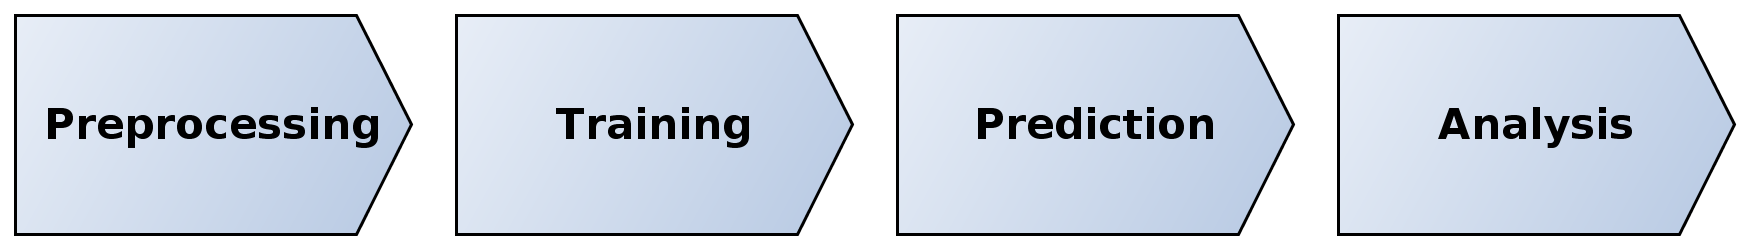
\includegraphics[width=0.85\textwidth]{images/allgemeinerAblauf}
  \caption{Einzelne Arbeitsschritte der Sprechererkennung}
  \label{fig:allgemeinerAblauf}
\end{figure}

\section{Preprocessing}
Der Schritt der Vorverarbeitung teilt sich in drei Teile auf: \emph{Konvertierung}, \emph{Feature Extraction} und \emph{Skalierung}. Diese drei Schritte werden in den folgenden Abschnitten genauer erläutert. Das Preprocessing ist von der Problemstellung abhängig. Bei der Sprechererkennung ist es die Verarbeitung von Audiostreams und die Abbildung auf die Stimm- und Hörorgane des Menschen.

\subsection{Konvertierung}
Mit der Konvertierung wird dafür gesorgt, dass die Daten im gleichen Format vorliegen. Für die Sprechererkennung reicht es, wenn die Audiodaten auf einen Kanal beschränkt werden (\emph{Mono}). Des Weiteren wird in dieser Projektarbeit eine Abtastrate von 16 kHz und einer Abtastgenauigkeit von 16 Bit verwendet.

\subsection{Feature Extraction}
Zur Extraktion von wichtigen Informationen werden zwei gängige Verfahren eingesetzt. Zum einen ist dies das Linear Predictive Coding (LPC). Beim LPC wird der Stimmtrakt des Menschen modellhaft nachgebildet. Dadurch wird die Datenbasis stark reduziert und werden nur die wichtigsten Informationen gespeichert.

Mel Frequency Cepstral Coefficients (MFCC)

\subsection{Skalierung}
Gelegentlich kann durch eine Skalierung der extrahierten Daten die Erkennung verbessert werden. Wahlweise kann zwischen $[0,1]$ oder $[-1,1]$ skaliert werden. Die Skalierung erfolgt linear nach der Formel \ref{equ:skalierung1} für $[0,1]$ und nach der Formel \ref{equ:skalierung2} für $[-1,1]$. $min$ stellt den kleinsten Wert der zu skalierenden Daten dar. $max$ den größten Wert. \cite{bib:svmfaq}
\begin{equation}
	\label{equ:skalierung1}
	x'=\frac{x-min}{max-min}
\end{equation}
\begin{equation}
	\label{equ:skalierung2}
	x'=2*\frac{x-min}{max-min}-1
\end{equation}

\section{Training}
Übersicht über Training, Weitere Möglichkeiten (K-Means, Kohonenkarten,...)
\subsection{Neural Gas}
Robustes Neuronales Netz
Nachbarschaftsreichweite
Update-Regel
\subsection{Support Vector Machine}
Support Vector Machine (SVM) ist ein (optimaler) Klassifikator
Eingesetzt wird Multi-Class SVM (One vs. One, One vs. Rest)

\section{Prediction}
Übersicht über Prediction, Erklärung Prediction = Arbeitsphase, erzeugt Ergebnis
\subsection{Nearest Neighbor}
Distanz zwischen Eingabevektor und Codebookvektoren
\subsection{Klassifikation}
Einordnung von Merkmalsvektoren

\section{Analysis}
Dient der Überprüfung des Ergebnisses der Prediciton-Phase evtl. mit Visualisierung\\
Möglichkeiten sind die absolute Erkennungsrate, Erkennungsrate auf mehrere Frames hintereinander, Verwechslungsmatrix
